% Chapter Template

\chapter{Introduction} % Main chapter title

\label{Chapter1} % Change X to a consecutive number; for referencing this chapter elsewhere, use \ref{ChapterX}

\lhead{Chapter 1. \emph{Introduction}} % Change X to a consecutive number; this is for the header on each page - perhaps a shortened title

%----------------------------------------------------------------------------------------
%	SECTION 1
%----------------------------------------------------------------------------------------
Robots have moved from being predominantly in factories to our daily lives. The flying drones doing surveillance, cleaning and serving robots, autonomous cars, and underwater vehicles are all common nowadays.

\section{Motivation and Objectives}

The legged robots have shown great potential in locomotion

\begin{figure}[!htb]
\centering
\begin{minipage}{.5\textwidth}
  \centering
  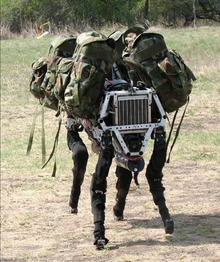
\includegraphics[width=0.65\linewidth]{bigdog.jpg}
  \caption*{(a) BigDog}
\end{minipage}%
\begin{minipage}{.5\textwidth}
  \centering
  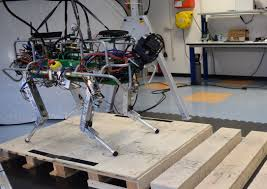
\includegraphics[width=1\linewidth]{hyq.jpeg}
  \caption*{(b) HyQ: Hydraulic Quadruped}
\end{minipage}
\caption[(a) Boston Dynamics' BigDog, (b) HyQ developed by IIT, Genoa, Italy]{(a) Boston Dynamics' BigDog which could carry upto 340 pounds at 4 miles per hour over a rough terrain, which was designed to support military operations, but had issues with noise which was audible from 4 miles away \citep{raibert2008bigdog}, (b) HyQ developed by IIT, Genoa, Italy\citep{semini2011design}}
\end{figure}


\section{Literature Review}

your content here .....\citep{greenwood1997classical}

Some assumption or definition explained in footnote\footnote{My footnote content here}.

\section{Outline}
The thesis focuses on the ....

Chapter \ref{Chapter2} introduces .... Chapter \ref{Chapter3} describes ...

Chapter \ref{Chapter4} focuses on the trajectory optimization .... Later in Chapter \ref{Chapter5}, the results obtained from .... Chapter \ref{Chapter6} provides the conclusion of the work along with the future scope.

